\section{Introduction}

Everyone with an interest in ice sheet modelling is encouraged to contribute
to GLIMMER. However, the structure of the model is complex, and the coding
style is more object-oriented than is generally common in geosciences
models. The aim of this chapter is to introduce these characteristics of the
model and to suggest some approaches to GLIMMER development. Detail is then
provided on some of the modules present within the GLIMMER code base.

In developing new code, several important principles should be borne in
mind. These are useful ideas when developing any code, but are especially
important when contributing to an established collaborative project like
GLIMMER:
\begin{itemize}
\item \textbf{Modularise/objectify.} Divide the code up into logically self-contained
  tasks. In a numerical model of a set of physical processes, this usually
  means taking each process separately, though of course the numerical
  techniques used will have a bearing on how the division is done --- implicit
  solutions of systems of equations require a more integrated
  approach. Objectification is covered in more detail below.
\item \textbf{Don't duplicate.} At all costs, avoid duplicating code within a
  model, as it makes bug-fixing and other maintenance nightmarish.
  Put it in a subroutine and call it from different places. Consider
  doing this even if the duplicated code is slightly different --- write the
  subroutine so it will do these different things.
\item \textbf{Don't reinvent the wheel.} If an existing piece of code in the
  model does what you need already, use it. If it nearly does what you need,
  extend it.
\item \textbf{Respect the hierarchy of the code.} Some parts of the model are
  `core', some are shared utility code, some are extensions/drivers/models of
  boundary conditions. Avoid creating a birds-nest of dependencies. If a piece
  of code from an extension acquires general usefulness, consider moving it to
  one of the shared utility modules.
\item \textbf{Write for flexibility.} The is almost never any justification
  for using static arrays (i.e. fixed sizes at compile-time), and certainly
  the size of an array should be defined at only one point in the
  code. Likewise, physical and other numerical parameters should be organised
  in a central place, and made configurable at runtime if there is a chance
  someone might want to change them. Think beyond what you're doing now to
  what you might want to do in the future, and write code accordingly.
\item \textbf{Be conservative.} Although radical restructuring or rewriting can
  sometimes be necessary, it should only be done after careful consideration
  of the potential consequences. Usually, incremental, gradual change is
  best. Also, when making changes, it's very important to retain the existing
  functionality and the form of the user interfaces (code interfaces and
  configuration options) if at all possible. Extend rather than alter.
\item \textbf{Write comments.} It's almost impossible to write too many
  comments in your code. It's especially important to document subroutine
  arguments, including the units of quantities, temporal validity,
  etc. Remember, in a few weeks' time, you'll probably have forgotten half of
  it, and will be glad of the comments\ldots
\item \textbf{Lay out your code neatly.} Indentation of code blocks and leaving blank lines
  between different sections of code are important ways to make code
  more readable. Most good editors have an automatic indentation facility ---
  Emacs is a good editor in this respect\footnote{Hint: if emacs doesn't enter
  the F90 edit mode immediately upon opening a file, you need to type \emph{Alt-}\texttt{x},
  followed by \texttt{f90-mode}, and press \emph{$<$enter$>$}.}.
\item \textbf{Use long, meaningful names.} There's not much virtue these days
  in making variable and subroutine names short and opaque --- we don't have
  issues with memory, and Fortran 90/95 allows names to be up to 31
  characters. It may involve a bit more typing to use long names, and care
  must be taken to ensure they don't get too long, but the extra time spent
  typing is worth it if the code actually means something when you look at it
  again a few weeks later.
\item \textbf{Use version control.} Although it takes a little time to learn
  to use a version control system, it really does make life easier. If you've
  ever got confused about which version of the code you or your collaborators
  have, or wished you could revert the changes you've just made, then you need
  version control. We use CVS for GLIMMER, but other systems are available. Of
  these, Subversion is generally seen as a promising alternative and successor
  to CVS.
\end{itemize}
The sections that follow cover some of these topics in more detail, but much
that passes for good-practice in code development is best learnt from
experience, and by looking at existing code.
%
\section{Introduction to GLIMMER programming techniques}
%
Although GLIMMER is written in Fortran, a very widely used language in the
geosciences, many of the techniques employed in the model will be unfamiliar
to even seasoned Fortran programmers. What follows is a brief description of
some of these more advanced techniques. For further information about the
topics covered, the reader is directed to \cite{Metcalf1999} and \cite{Decyk1997}.
%
\subsection{Fortran Modules}
%
\subsubsection{Module definition}
%
The basic building block of the GLIMMER structure is the Fortran 90/95 module,
which is a way of collecting together subroutines, functions type definitions
and variables into a single scope\footnote{A \emph{scope} or \emph{namespace}
 is the term for the program unit where a given \emph{name}, such as a variable
 or subroutine name, is valid. For instance, if a variable is declared at the
 beginning of a subroutine, the body of the subroutine is that variable's
 scope; outside the scope, the name is undefined, or may be defined
 differently.}. The module may then be used within another piece of code, so that the
names in the modules scope are available in the other piece of code. A module
block is defined like this:
%
\begin{alltt}
    module \textrm{\textit{module-name}}

        \textrm{\textit{module variable declarations}}
        \textrm{\textit{derived-type definitions}}

    contains

        \textrm{\textit{function and subroutine declarations}}

    end module
\end{alltt}
%
The \texttt{contains} is omitted if no subroutines or functions are
present. It is good practice to put each module in a separate file, and give
the filename the same name as the module.
%
\subsubsection{Using modules}
%
A module is accessed by another piece of code with the \texttt{use}
statement. Thus, if the module \texttt{foo} contains the subroutine
\texttt{bar}, another piece of code may make use of it in this way:
%
\begin{alltt}
    program \textrm{\textit{program-name}}

        use foo

        implicit none

        \textrm{\textit{variable declarations}}

        call bar

    end program \textrm{\textit{program-name}}
\end{alltt}
%
Of course, subroutines, functions and modules can all contain \texttt{use}
statements as well.
%
\subsubsection{Privacy in modules}
%
By default, all the names in a module's scope become available to any program
element that references it with a \texttt{use} statement. There are
circumstances where this is undesirable, and so Fortran 90/95 provides a way
to define names as public or private. The \texttt{public} and \texttt{private}
statements may both be present in the first block of a module (i.e. before the
\texttt{contains}, if present). The list of variable and/or subroutine names
follows. For example:
%
\begin{alltt}
    private :: foo, bar, blah
\end{alltt}
%
It is good practice to be clear about what parts of a module form a public
interface, and define this formally. A good way of doing this is to set the
default to private, and then set specific names as public:
%
\begin{alltt}
    private
    public :: foo, bar
\end{alltt}
%
This technique is useful for avoiding name conflicts when two modules might
define internal variables or subroutines with the same name (e.g. \texttt{pi}
for the value of
$\pi$). Also, public subroutines are best named in an un-generic way, by
prefixing their names with the name of the module. For instance, the module
\texttt{glimmer\_daily\_pdd} contains the public subroutines
\texttt{glimmer\_daily\_pdd\_init} and \texttt{glimmer\_daily\_pdd\_mbal}.
%
\subsection{Derived types}
%
A derived type is a way of collecting together an arbitrary set of
variables and arrays into a composite variable type, instances of which can be addressed with a
single name. The concept of derived types takes us some way towards so-called
object-oriented programming (OOP) techniques, though there are some important
OOP techniques that are not implemented in Fortran 90/95.

A derived type is defined in this kind of way:
\begin{alltt}
    type typename
        real :: realvar
        integer :: intvar
        real,pointer,dimension(:,:) :: realarr => null()
    end type typename
\end{alltt}
So, a derived type can contain any scalar variables, and also pointers (either
scalar pointers or array pointers). Fortran 90/95 does not permit derived type
elements to be allocatable arrays, but since the behaviour of pointer arrays
is very similar, this isn't a serious problem.

The type definition doesn't actually create any variables though. To do that,
you need to use the \texttt{type} declaration to create an instance of the
derived type (known as a \emph{structure}), just as with any other type of
variable:
%
\begin{alltt}
    type(typename) :: fred, jim, bob
\end{alltt} 
%
This creates three structures of type \texttt{typename}, called \texttt{fred},
\texttt{jim} and \texttt{bob}. Structures can be handled like ordinary
variables, and passed to subroutines in argument lists, etc. The individual
elements may be addressed using the \texttt{\%} operator:
%
\begin{alltt}
    fred%realvar = 4.5
    jim%intvar = fred%intvar + 7
    allocate(bob%realarr(nx,ny))
\end{alltt}

Note that by default, mathematical operators have no meaning when applied to
derived types; writing \texttt{bob = fred + jim} isn't allowed. If you want to
add the elements of \texttt{fred} to the elements of \texttt{jim}, it's
necessary to write a function to do so, so that you would, for example, write
\texttt{bob = typename\_add(fred,jim)} It is possible to define the meaning of
the \texttt{+} operator so that it uses the function \texttt{typename\_add} to
perform the addition (a process known as \emph{operator overloading}), but
describing how is beyond the scope of this document. In any case, derived types
in GLIMMER are not generally used in a way such that arithmetic operations
would make sense.

Usually, derived type definitions are put into modules (before
\texttt{contains}), so that they can easily be used in different pieces of
code. The power that this combination of type definitions and modules gives is
described in the next section.
%
\subsection{Object-orientation with modules and derived types}

As the name implies, the \emph{object} is the central concept of
object-oriented programming. In traditional OOP terminology, a \emph{class}
defines a type of object. The class has particular \emph{attributes}, which
might be numerical values, strings or whatever (i.e. they're variables that
are part of the class), and \emph{methods}, which are things you can ask an
object to \emph{do} to itself (i.e. methods are functions or subroutines which
are part of a class).

Explaining OOP with examples is notoriously tricky because the easiest
examples of classes are those that mirror classes of objects in the real
world, but this inevitably seems a bit contrived. So, although it seems a bit
ridiculous, here's one such example\ldots Imagine a class which describes a
domestic oven. What are the attributes of an oven, that differentiate one oven
from another? These could be the size of the oven, it's type (electric or
gas), as well those things that describe its present state: the thermostat
setting, the actual oven temperature, whether the heating element is on or
off, and whether the door is open or not

Secondly, what kind of actions can we perform on the oven? Most likely, we
want to be able to open and close the oven door, check the present
temperature, and set the thermostat. These actions are the methods.

In terms of Fortran 90, we can use the mechanism of modules and derived types
to implement a somewhat limited form of OOP:
%
\begin{alltt}
  module domestic_oven

    type oven
      real :: width,height,depth
      real :: thermostat
      real :: temperature
      logical :: element      ! .true. for no, .false. for off
      logical :: door         ! .true. for open, .false. for closed
      character(10) :: oven_type
    end type oven

  contains

    subroutine oven_set_thermostat(self,temp)

      type(oven) :: self
      real :: temp

      self%temperature = temp

    end subroutine oven_set_thermostat

    \textrm{\textit{\ldots plus other functions/subroutines}}

  end module domestic_oven
\end{alltt}
%
A module like this will usually include a subroutine to initialise objects; in
this case, you would expect to be able to specify the size of the oven, its
type, initial temperature, etc.

So much for computer models of domestic ovens; what use is OOP to ice
modellers? Well, using the technique described above is what allows GLIMMER to
be used to run several regional ice models simultaneously. It also makes
adding new mass-balance models to GLINT much easier. In fact, the principles
of OOP are used all over the GLIMMER code, so it is worth getting to grips
with them.
%
\subsection{Example of OOP in Glimmer}
%
A good, self-contained example of GLIMMER programming style, and the use of
OOP is the way that the daily PDD mass-balance scheme (in
\texttt{glimmer\_daily\_pdd.F90}) has been implemented. Here, the parameters
of the scheme are stored in the derived type
\texttt{glimmer\_daily\_pdd\_params}, and the public interface of the module
is limited to this derived type, and two subroutines
(\texttt{glimmer\_daily\_pdd\_init} and
\texttt{glimmer\_daily\_pdd\_mbal}). Everything else is kept private within
the module. The initialisation subroutine uses the standard GLIMMER configuration
file reader to get input parameters, and the GLIMMER logging mechanism to
output data to the screen and/or file. The object-like structure means that it
is easy to use the daily PDD model within some other piece of code: all one
needs to do is declare an instance of \texttt{glimmer\_daily\_pdd\_params},
initialise it appropriately, and then call the
\texttt{glimmer\_daily\_pdd\_mbal} subroutine. Also, although the PDD model is
currently initialised from file, it would be easy to write an
alternative initialisation routine within the module to get the parameters
from a subroutine argument list, extending the capabilities of the module
rather than changing the present interface.
%
\subsection{Pointers}
%
The final more advanced topic covered here is the Fortran pointer. Thankfully,
the name is self-explanatory --- a pointer is a thing that points to another
thing. This might not sound like much use, but since pointers can be made to
point at different things as the program runs, and can have memory allocated
for them to point to, they can be used to create flexible, dynamic data
structures. The thing that a pointer points to is called a \emph{target}.
%
\subsubsection{Pointer basics}
%
Pointers are declared much like an ordinary variable, but with the \texttt{pointer}
attribute. For example, to declare an integer pointer, one would write this:
%
\begin{alltt}
    integer, pointer :: foo => null()
\end{alltt}
%
The second part of this statement (\texttt{=>null()}) initialises the pointer
to null (i.e. pointing to nothing). This is only available in Fortran 95, but
it is highly desirable to use it, as otherwise the pointer's target is
undefined\footnote{\emph{Undefined} is not the same thing as pointing at
  nothing. Undefined pointers can cause a program to crash very easily; the
  lack of null initialisation in Fortran 90 is one of the more serious
  omissions that Fortran 95 sought to address.}.

Note that although we have declared a pointer with this statement, we can't
use it as a variable yet, as it isn't pointing at an integer-sized chunk of
memory. There are two ways of rectifying this: either the pointer can be made
to point to an existing variable, or a new block of memory
can be allocated to hold the target. These two methods are known as
\emph{pointer assignment} and \emph{pointer allocation}, respectively.
%
\subsubsection{Pointer assignment}
%
Pointing a pointer at something is very simple. The pointer assignment
statement uses the \texttt{=>} operator:
%
\begin{alltt}
    a => b
\end{alltt}
%
This statement sets pointer \texttt{a} to point to target \texttt{b}. For this
to be valid Fortran, \texttt{a} must have the \texttt{pointer} attribute,
while \texttt{b} must be either a variable with the \texttt{target} attribute,
or another pointer. If the target is a pointer, then the first pointer is set
to point at the second pointer's target. This means that
%
\begin{alltt}
    a => b
    c => a
\end{alltt}
%
is equivalent to
%
\begin{alltt}
    a => b
    c => b
\end{alltt}
%
\subsubsection{Pointer allocation}
%
A pointer can be made to point to a newly-allocated chunk of memory using the
\texttt{allocate} statement, in the same way as an allocatable array is
handled:
%
\begin{alltt}
    allocate(a)
\end{alltt}
%
By using the pointer assignment described above, other pointers may be made to
point at the same piece of memory:
%
\begin{alltt}
    b => a
\end{alltt}
%
\subsubsection{Un-pointing pointers, and avoiding memory leaks.}
%
A pointer can be nullified (made to point to nothing) in two ways: using the
\texttt{null} function, or the nullify statement:
%
\begin{alltt}
    p => null()
    nullify(p)
\end{alltt}
%
Care has to be taken with this, however. Recall the memory allocation example given above:
%
\begin{alltt}
    allocate(a)
    b => a
\end{alltt}
%
It is significant that the memory location that \texttt{a} and \texttt{b} now point to
doesn't have a name of its own, which means that if \texttt{a} and \texttt{b}
are subsequently both made to point to something else, or to nothing, the
target variable becomes impossible to recover. Consider this sequence of
two statements:
%
\begin{alltt}
    allocate(a)
    a => null()
\end{alltt}
%
Here, a block of memory is allocated, and \texttt{a} is made to point to
it. Then, \texttt{a} is made to point to nothing. However, the block of memory
allocated in the first statement hasn't been deallocated, and is now
unrecoverable --- and unusable --- since we don't have a name to refer to it by.
This is known as a \emph{memory leak}, and it is a Bad Thing. It's not
disastrous if a few integer-sized blocks of memory suffer this fate, but if
large amounts of memory are lost like this, it is quite possible for the
program to crash or become very slow as a result.

The proper way to avoid memory leaks is to deallocate memory before it becomes
dereferenced, using the \texttt{deallocate} statement\footnote{It's not clear
  to me whether the assignment of \texttt{a} to \texttt{null} is necessary in
  this example. Some compilers take it as read that if a block of memory that
  a pointer points to is deallocated, that pointer is also nullified, but I am
not sure if this is universal.}:
%
\begin{alltt}
    allocate(a)
    deallocate(a)
    a => null()
\end{alltt}
%
 The reason that this isn't done automatically when a pointer is nullified is because there may be
other pointers still pointing to that memory location. The process of working
out which chunks of memory have been `orphaned' and so need to be deallocated
(known as \emph{garbage collection}) is complex, and compiled languages like
Fortran don't usually do it automatically. Avoiding memory leaks therefore
depends on careful program design.
%
\subsubsection{Linked lists}
%
A major use for pointers is the linked list, a flexible data structure whose
size and structure can be changed dynamically, without having to reallocate it
from scratch (which is the case with allocatable arrays).

The principle of the linked list is that each element of the list points to
the next element. Extra elements can be added to the end of the list by
allocating more memory, and making the final element point to it. Other
actions can be done by manipulating the pointers of the various elements.

A typical linked list might use the following derived type:
%
\begin{alltt}
    type list
        type(list) :: next => null()
        type(list) :: previous => null()
        integer :: value
    end type list
\end{alltt}
%
So, the type contains pointers that point to the next and previous elements
of the list. Describing how to implement subroutines and functions to
construct, read and modify the list is beyond the scope of this document, but
a full example is provided in \cite{Metcalf1999}.

GLIMMER makes several uses of linked lists and pointer techniques, most
notably in the handling of configuration and output files.
%
\section{GLIMMER structure and design}
%
\subsection{Overview}
%
The `design' of GLIMMER is a consequence of the way it has been
developed. Initially, as a stand-alone model with a single domain, module
variables were used to hold all model fields and parameters. With the move to
use GLIMMER as the ice model component within GENIE, and the desire to enable
several active regions to be run simultaneously, the module variables were
converted into components of derived types, and an extra layer added on top of
the existing structure to deal with global fields and parameters, and deal
with the downscaling/interpolation of input fields. A subsequent major
reorganisation then allowed the use of the ice model in stand-alone mode
again, and the present GLINT-GLIDE structure was born. Doubtlessly, the
resulting structure is more complex than necessary, but hopefully it is still
reasonably logical.

Currently (July 2006), the \texttt{fortran} directory in the GLIMMER source
tree contains 83 \texttt{.F90} files, including automatically generated
NetCDF IO files (more on this below). Figure~\ref{ug.fig.glimmer} indicates
the general relationship between the various parts of GLIMMER; a more
comprehensive overview, with filename patterns, is shown in
figure~\ref{dg.fig.glimmer_structure}. 
%
\begin{figure}[htbp]
  \centering
  \includegraphics[width=0.85\textwidth]{\dir/figures/glimmer_structure.eps}
  \caption{Relationship between the various GLIMMER components, giving
  filenames and dependencies. The modules in GLUM are used by all other
  elements of the diagram.}
  \label{dg.fig.glimmer_structure}
\end{figure}
%
The various parts of GLIMMER shown in the diagram are as follows:
%
\begin{itemize}
\item \textbf{GLIDE} (\textbf{GL}IMMER \textbf{I}ce \textbf{D}ynamics
  \textbf{E}lement). This is the core ice model, whose core interface consists
  of a derived type definition, and a small number of subroutines to
  initialise the model, perform time steps and tidy up at the end. In the most
  basic set up, all that needs to be supplied to GLIDE is the surface
  mass-balance and surface air temperature fields.
\item \textbf{GLUM} (\textbf{GL}IMMER \textbf{U}seful \textbf{M}odules). These
  are modules that contain code which is used by all the other parts of
  GLIMMER. Some of these (for instance, the configuration parser, NetCDF IO
  and logging system) are of general use to any model built on top of
  GLIMMER.
\item \textbf{Isostasy model.} Although currently only used by GLIDE, the
  isostasy model is written in such a way as to be easily coupled to another
  ice model if necessary. Probably this should be moved to within GLUM,
  though?
\item \textbf{Climate drivers.} The flexibility of GLIMMER comes from the ease
  with which GLIDE may be coupled to a custom climate driver. A number of
  these are provided as part of the GLIMMER code base:
\begin{itemize}
\item \textbf{Simple driver.} This is essentially an example driver, almost as simple
  as possible in design. It is used to implement the idealised EISMINT 1
  tests.
\item \textbf{Edinburgh Ice Sheet driver (EIS).} This is a driver based on the
  Edinburgh Model (see \cite{Hagdorn2003}, for example).
\item \textbf{EISMINT 3 Greenland.} This driver implements the Greenland test
  cases from the second phase of the EISMINT project (termed EISMINT 3 to
  distinguish it from the second part of the first EISMINT project\ldots)
\item \textbf{GLINT} (\textbf{GL}IMMER \textbf{Int}erface). This complex
  driver is designed to form an interface between GLIDE and a global climate
  model. Originally developed for the GENIE project, it can be used in
  conjunction with any global model defined on a lat-lon grid. GLINT has its
  own complex structure of derived types, described below, and is itself
  supplied with two example climate drivers, \texttt{glint\_example} and \texttt{glex\_ebm}.
\end{itemize}
\end{itemize}
%
\subsection{GLIDE structure}
%
GLIDE is the heart of GLIMMER, the ice dynamics model. The top-level class or
derived type is \texttt{glide\_global\_type}, and this contains instances of
other derived types, some defined within GLIDE, others within GLUM. The
situation is summarised in figure~\ref{dg.fig.glide_class_diagram}. All GLIDE
derived types are defined in \texttt{glide\_types.F90}; the others are defined
within various GLUM files as shown.
%
\begin{figure}[htbp]
\centering
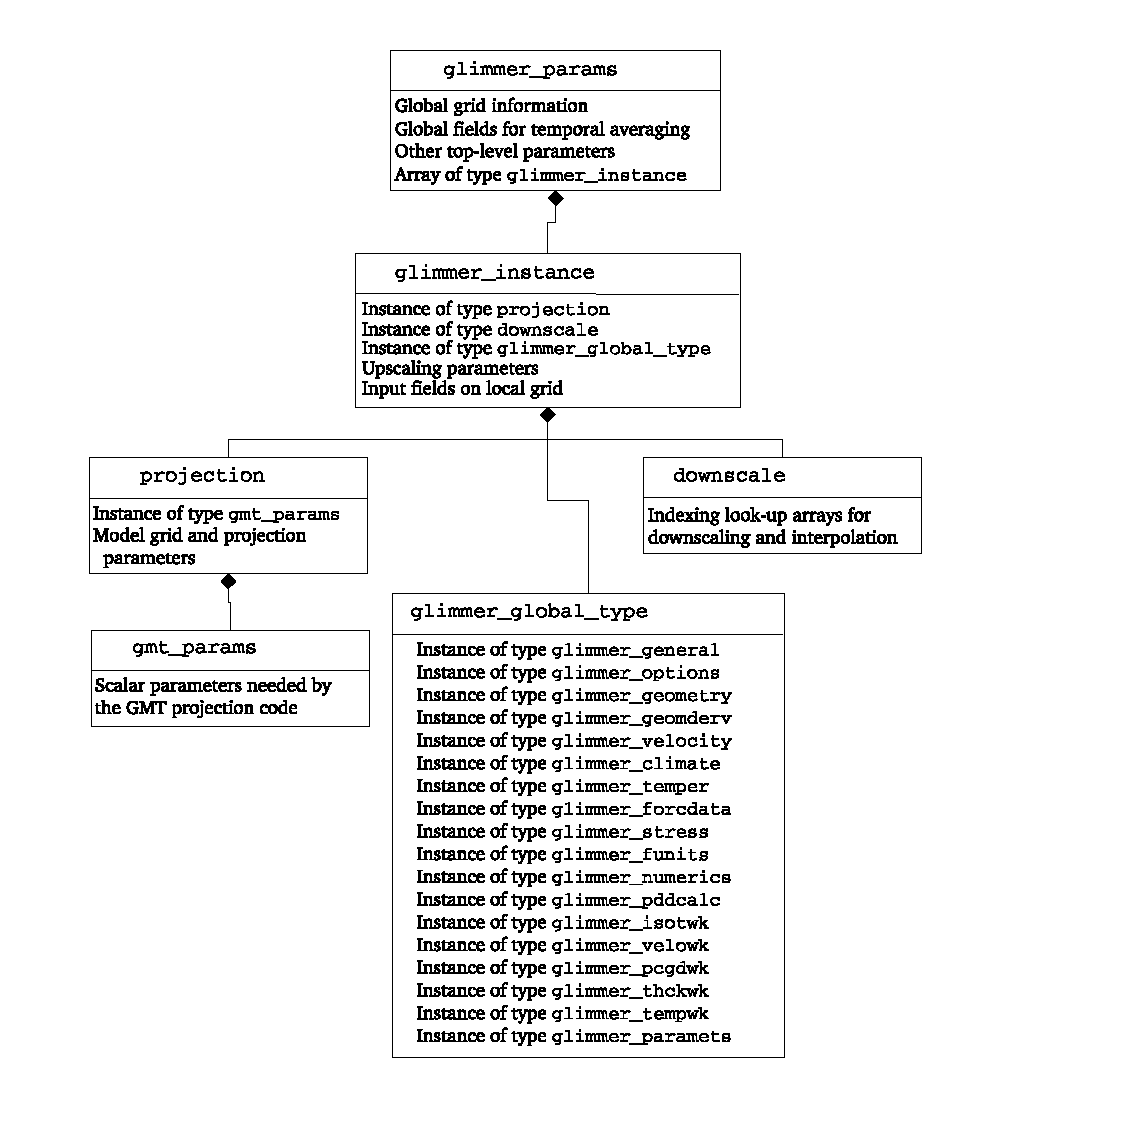
\includegraphics[width=\textwidth]{\dir/figures/class_diagram.eps}
\caption{Main `Class Diagram' for GLIDE, in quasi-UML notation. Only derived type components which
  are themselves derived types are shown; intrinsic type components are
  omitted. Also omitted are derived types which are defined within GLIDE but
  which contain no derived type components. Derived types in GLUM are
  coloured to show which file they are defined in.}
\label{dg.fig.glide_class_diagram}
\end{figure}

In addition to the relationships illustrated in
figure~\ref{dg.fig.glide_class_diagram}, there is a web of dependencies based
on module \texttt{use} statements. This structure is too complex to be
illustrated in a dependency diagram; figure~\ref{dg.fig.glide_mod_depend} shows the direct module
dependencies of module \texttt{glide}.
%
\begin{figure}[htbp]
\centering
\includegraphics[width=\textwidth]{\dir/figures/glide_mod_depend.eps}
\caption{Direct module dependency diagram for module \texttt{glide} only,
  illustrating the complexity of module dependencies.}
\label{dg.fig.glide_mod_depend}
\end{figure}

A brief description of the modules and files that comprise GLIDE is given here:
\begin{center}
  \tablefirsthead{%
    \hline
  }
  \tablehead{%
    \hline
    \multicolumn{3}{|p{0.98\textwidth}|}{\emph{\small continued from previous page}}\\
    \hline
  }
  \tabletail{%
    \hline
    \multicolumn{3}{|r|}{\emph{\small continued on next page}}\\
    \hline}
  \tablelasttail{\hline}
  \begin{supertabular}{|l|l|p{7cm}|}
    Module name & Filename & Description \\
    \hline
    \hline
    \texttt{glide} & \texttt{glide.F90} & Top-level GLIDE module. Contains
    subroutines to read a config file, initialise the model, and perform
    time-steps.\\
    \texttt{glide\_io} & \texttt{glide\_io.F90} & NetCDF IO routines for
    GLIDE. This file is auto-generated (see below).\\
    \texttt{glide\_lithot} & \texttt{glide\_lithot.F90} & Top-level module for
    lithosphere temperature/heat-flux model. \\
    \texttt{glide\_lithot1d} & \texttt{glide\_lithot1d.F90} & One-dimensional
    model for lithosphere temperature calculations. Used by \texttt{glide\_lithot}.\\
    \texttt{glide\_lithot3d} & \texttt{glide\_lithot3d.F90} & Three-dimensional
    model for lithosphere temperature calculations. Used by \texttt{glide\_lithot}.\\
    \texttt{glide\_mask} & \texttt{glide\_mask.F90} & Contains code to
    determine the properties of each grid-box --- whether ice is present,
    whether it is floating, is a marine margin cell, etc. The output for each
    cell is a number whose bits each represent a different property. \\
    \texttt{glide\_nc\_custom} & \texttt{glide\_nc\_custom.F90} & Code to
    write contents of dimension variables (\texttt{x1}, \texttt{x0}, etc.) to
    output NetCDF file.\\
    \texttt{glide\_profile} & \texttt{glide\_profile.F90} & Wrapper for
    \texttt{profile.F90} (determines how much processor time is devoted to
    each task) with GLIDE-specific configuration. Useful for
    debugging/analysis. \\
    \texttt{glide\_setup} & \texttt{glide\_setup.F90} & Subroutines used in
    GLIDE initialisation (reading configuration files, etc). Also contains a
    few bits of code used by the model each time step, that should properly be
    located somewhere else (\texttt{glide\_maskthck},
    \texttt{glide\_marinlim} and \texttt{glide\_calclsrf}).\\
    \texttt{glide\_stop} & \texttt{glide\_stop.F90} & Module for tidying up at
    the end of a model run (contains only subroutine \texttt{glide\_finalise}).\\
    \texttt{glide\_temp} & \texttt{glide\_temp.F90} & GLIDE ice thermodynamics
    code. \\
    \texttt{glide\_thck} & \texttt{glide\_thck.F90} & Thickness evolution
    code. \\
    \texttt{glide\_types} & \texttt{glide\_types.F90} & Definitions of all
    GLIDE derived types (see figure~\ref{dg.fig.glide_class_diagram}).\\
    \texttt{glide\_velo} & \texttt{glide\_velo.F90} & Code for GLIDE ice
    velocity calculations. \\

  \end{supertabular}
\end{center}

\subsection{GLINT structure}
%
As the most complex of the driver programs supplied as part of GLIMMER, the
structure of GLINT is described next. As with GLIDE, on which it is built, the
GLINT structure uses a hierarchy of derived types, shown in
figure~\ref{dg.fig.glint_class_diagram}. The most significant aspect of this
diagram is that the top-level type (\texttt{glint\_params}) contains the
parameters that are relevant to the coupling on a global level, including an
array (\texttt{instances}) of type \texttt{glint\_instance}. Each element of
this array contains a single GLIDE model instance. The reason for using a
wrapper type, rather than having an array of type \texttt{glide\_global\_type},
is that there is a lot of instance-specific information (the mass-balance
model, downscaling/upscaling, etc.) that isn't contained in the GLIDE derived
type.

There is some redundancy in this data structure, which should be corrected at
some point in the future. Most significant is the presence in both GLIDE and
GLINT of data structures describing the map projection of the model. (types
\texttt{projection} and \texttt{CFproj\_projection}). GLINT uses the former to
work out where the model instance is on the globe, and obtains the information
from the configuration file; GLIDE reads and writes the latter from the NetCDF
files, but doesn't use the information for calculation. Currently, there is no
coordination between the two sets of information. 
%
\begin{figure}[htbp]
\centering
\includegraphics[width=\textwidth]{\dir/figures/class_diagram_glint.eps}
\caption{GLINT `class diagram', in quasi-UML notation. Only derived type components which
  are themselves derived types are shown; intrinsic type components are
  omitted. The top-level GLIDE type is shown in yellow.}
\label{dg.fig.glint_class_diagram}
\end{figure}

The modules comprising GLINT are as follows:
\begin{center}
  \tablefirsthead{%
    \hline
  }
  \tablehead{%
    \hline
    \multicolumn{3}{|p{0.98\textwidth}|}{\emph{\small continued from previous page}}\\
    \hline
  }
  \tabletail{%
    \hline
    \multicolumn{3}{|r|}{\emph{\small continued on next page}}\\
    \hline}
  \tablelasttail{\hline}
  \begin{supertabular}{|l|l|p{7cm}|}
    Module name & Filename & Description \\
    \hline
    \hline
    \texttt{glint\_main} & \texttt{glint.F90} & Top-level GLINT module -
    public subroutines initialise model, perform a time step, and finalise the
    model at a global level. Other modules deal with individual GLINT
    instances.
    Temporal averaging of global input fields and collation of upscaled
    output takes place in this module. \\
    \texttt{glint\_climate} & \texttt{glint\_climate.F90} & Various
    subroutines used to process the GLINT climate. Includes climate field
    downscaling and lapse-rate correction. \\
    \texttt{glint\_constants} & \texttt{glint\_constants.F90} & Various
    constants used by GLINT but not GLIDE. Mostly relate to sub-year timescales.\\
    \texttt{glint\_global\_grid} & \texttt{glint\_global\_grid.F90} & Derived
    type that defines a global lat-lon grid, and subroutines to handle it. \\
    \texttt{glint\_global\_interp} & \texttt{glint\_global\_interp.F90} &
    Utility code to regrid data from one global grid to another, taking into
    account spherical geometry. \\
    \texttt{glint\_gmt} & \texttt{glint\_gmt.F90} & Code adapted from the
    Generic Mapping Tools (GMT), used for map projection handling.\\
    \texttt{glint\_initialise} & \texttt{glint\_initialise.F90} & Module used
    to initialise a GLINT instance (type \texttt{glint\_instance}). \\
    \texttt{glint\_interp} & \texttt{glint\_interp.F90} & Code to upscale and
    downscale between global and local grids. \\
    \texttt{glint\_io} & \texttt{glint\_io.F90} & GLINT NetCDF IO
    routines. Automatically-generated (see below). \\
    \texttt{glint\_mbal\_coupling} & \texttt{glint\_mbal\_coupling.F90} & This
    module coordinates the temporal accumulation of mass-balance quantities.\\
    \texttt{glint\_mbal} & \texttt{glint\_mbal.F90} & A wrapper for different
    mass-balance schemes --- gives them a common interface. \\
    \texttt{glint\_mbal\_io} & \texttt{glint\_mbal\_io.F90} & Auto-generated
    NetCDF IO routines for GLINT mass-balance calculations. \\
    \texttt{glint\_precip\_param} & \texttt{glint\_precip\_param.F90} & Implementation of the
    precipitation downscaling parameterization of Roe \& Lindzen. \\
    \texttt{glint\_proj} & \texttt{glint\_proj.F90} & Derived type definition
    and handling code for map projections. \\
    \texttt{smb\_dummy} & \texttt{glint\_smb.F90} & Dummy module in place of
    externally-connected RAPID energy-balance mass-balance model. \\
    \texttt{glint\_timestep} & \texttt{glint\_timestep.F90} & GLINT instance
    timestep code. \\
    \texttt{glint\_type} & \texttt{glint\_type.F90} & Definition of GLINT
    instance type. \\
  \end{supertabular}
\end{center}



\section{Physics documentation}

\subsection{Ice temperature evolution routines}

\subsubsection{Summary}
Call structure (filenames in brackets).
\begin{itemize}
    \item subroutine testinisthk [glimmer\_setup] and
    \item subroutine glimmer\_i\_tstep [glimmer\_object] call
    \item subroutine timeevoltemp [glimmer\_temp] calls
    \item subroutine calcartm [glimmer\_temp] and
    \item subroutine timeders [glimmer\_thck] and
    \item subroutine gridwvel [glimmer\_velo] and
    \item subroutine wvelintg [glimmer\_velo] and
    \item subroutine chckwvel [glimmer\_velo] and
    \item subroutine finddisp [glimmer\_temp] and
    \item subroutine hadvall [glimmer\_temp] and
    \item subroutine hadvpnt [glimmer\_temp] and
    \item subroutine findvtri [glimmer\_temp] and
    \item subroutine tridag [glimmer\_temp] and
    \item subroutine corrpmpt [glimmer\_temp] and
    \item subroutine swapbndt [glimmer\_temp] and
    \item subroutine calcbmlt [glimmer\_temp] and
    \item subroutine calcflwa [glimmer\_temp]
\end{itemize}

\noindent Modules used.
\begin{itemize}
    \item
\end{itemize}

\subsubsection{Introduction}
The section describes the routines that are concerned with
calculating the three-dimensional distribution of temperature
within the ice mass.  They can be broken down into five groups.
\begin{itemize}
    \item determining air temperature (upper boundary
    condition) [\texttt{calcartm}];
    \item determining vertical velocity field from existing
    horizontal velocity fields (normally only needed if temperature is being calculated) [\texttt{wvelintg}, chckwvel];
    \item routines associated with vertical grid coordinate
    system [\texttt{gridwvel}, \texttt{timeders}];
    \item the main temperature solver [\texttt{finddisp, hadvall, hadvpnt, findvtri, tridag, corrpmpt, swapbndt}];
    \item ancillary calculations that only make sense if temperature is being calculated
    [\texttt{calcbmlt}, \texttt{calcflwa}].
\end{itemize}

The basic quantity returned is a three-dimensional grid of
temperature in $\circ^{-1}$C (uncorrected for variations in
pressure melting point and unscaled).  Temperature is held in the
array \texttt{temp} and will be referred to here using the symbol
$T$.

In addition to temperature a number of other quantities are
calculated by these routines.  They include: basal melt rate ($m$
\texttt{bmlt} m yr$^{-1}$ scaled using \texttt{thk0/tim0}); basal
water depth ($W$ \texttt{bwat} m scaled using \texttt{thk0});
vertical velocity ($w$ \texttt{wvel} m yr$^{-1}$ scaled using
\texttt{thk0/tim0}); vertical velocity of numerical grid ($w_0$
\texttt{wgrd} m yr$^{-1}$ scaled using \texttt{thk0/tim0}); Glen's
A ($A$ \texttt{flwa} Pa$^{-3}$ yr$^{-1}$ scaled using
\texttt{vis0}); air temperature ($T_a$ $\circ^{-1}$C unscaled).
All scales are held in the module \texttt{paramets} in
\textbf{\texttt{glimmer\_paramets}}.

Three options are currently available for calculating $T$. The
particular option chosen is controlled by the input parameter
\texttt{whichtemp} (\texttt{gln} file).

\begin{description}
    \item[0] Set whole column to the appropriate surface air temperature ($T_a$).
    \item[1] This option is the main solver that determines temperature
    at the new time step from the appropriate three-dimensional
    advection-diffusion equation.
    \item[2] Set the upper surface temperature to $T_a$ and do a linear
    interpolation from this value to 0 $^\circ$C at the lower
    surface. Check for pressure melting and adjust any
    temperatures that are above melting point.
\end{description}

The subroutine \texttt{timeevoltemp} controls calculation of the
$T$ etc. It is called in the main time loop in
\textbf{\texttt{glimmer\_object}} and resides in
\textbf{\texttt{glimmer\_temp}}.
\section{Configuration File Parser}\label{dg.sec.config_file}
The run--time behaviour of the ice sheet model is controlled by configuration files. The old file format is based on Fortran namelists. The new configuration file format is loosely based on the format of Windows \texttt{.ini} files with sections containing name/value pairs. The new format is more flexible and can be easily understood by reading the configuration files. This section contains a description of the configuration file parser API.

\subsection{File Format}
The parser assumes a maximum number of 250 characters per line. Leading and trailing white space is ignored. Names are case sensitive.
\begin{description}
\item[Comments:] Empty lines and lines starting with \texttt{!}, \texttt{;} or \texttt{\#} are ignored.
\item[Sections:] Section names are enclosed with square prackets, \texttt{[]} and can be 20 character long.
\item[Parameters:] Parameter names are separated from their associated values with either \texttt{:} or \texttt{=}. The names can be 20 characters long. Values can be 200 characters long.
\end{description}

An example configuration file:
\begin{verbatim}
;a comment
[a section]
an_int  : 1
a_float = 2.0
a_char  = hey, this is rather cool
an_array = 10. 20. -10. 40. 100.

[another section]
! more comments
foo : bar
\end{verbatim}

\subsection{Architecture Overview}
The configuration data is stored as linked list. Each section is described by the following list element:
\begin{verbatim}
  type ConfigSection
     character(len=namelen) :: name
     type(ConfigValue), pointer :: values=>NULL()
     type(ConfigSection), pointer :: next=>NULL()
  end type ConfigSection
\end{verbatim}
The parameter name/value pairs defined in each section are stored in another linked list:
\begin{verbatim}
  type ConfigValue
     character(len=namelen) :: name
     character(len=valuelen) :: value
     type(ConfigValue), pointer :: next=>NULL()
  end type ConfigValue
\end{verbatim}
These linked lists are setup and read using subroutines.

\subsection{API}
\begin{description}
\item[Reading configuration files] Configuration files are read using \texttt{ConfigRead}. This subroutine parses the configuration file and populates the linked lists.
\begin{verbatim}
subroutine ConfigRead(fname,config)
  character(len=*), intent(in) :: fname
  type(ConfigSection), pointer :: config
end subroutine ConfigRead
\end{verbatim}
The pointer \texttt{config} contains the first section of the configuration file.
\item[Dumping configuration] The subroutine \texttt{PrintConfig} traverses the linked lists and prints them to standard output.
\begin{verbatim}
subroutine PrintConfig(config)
  type(ConfigSection), pointer :: config
end subroutine PrintConfig(config)
\end{verbatim}
\item[Searching for a Section] The subroutine \texttt{GetSection} can be used to find a specific section.
\begin{verbatim}
subroutine GetSection(config,found,name)
  type(ConfigSection), pointer :: config
  type(ConfigSection), pointer :: found
  character(len=*),intent(in) :: name
end subroutine GetSection
\end{verbatim}
On exit the pointer \texttt{found} will point to the first section called \texttt{name}. \texttt{found} points to \texttt{NULL()} if the section \texttt{name} is not found.
\item[Reading parameters] Paramter name/value pairs are found using the \texttt{GetValue} family of subroutines. \texttt{GetValue} provides an interface to the individual subroutines \texttt{GetValueChar}, \texttt{GetValueInt}, \texttt{GetValueReal}, \texttt{GetValueIntArray} and \texttt{GetValueRealArray}.
\begin{verbatim}
subroutine GetValue(section,name,val)
  type(ConfigSection), pointer :: section
  character(len=*),intent(in) :: name
  sometype :: val
  integer,intent(in), optional :: numval
end subroutine GetValue
\end{verbatim}
\texttt{section} is the section that should be searched for the parameter \texttt{name}. On exit \texttt{val} contains the parameter value if it is found, otherwise it is unchanged. 

The array versions of \texttt{GetValue} expect value to be a pointer to a one--dimensional array. \texttt{val} is deallocated if it was allocated on entry. The array versions of \texttt{GetValue} also accept an optional value, \texttt{numval}, with which the maximum number of array elements can be set. The default is 100. Array elements are separated by white space.
\end{description}

\section{netCDF I/O}
The netCDF\footnote{\texttt{http://www.unidata.ucar.edu/packages/netcdf/}} library is used for platform independent, binary file I/O. GLIMMER makes use of the f90 netCDF interface. The majority of the source files are automatically generated from template files and a variable definition file using a python script. The netCDF files adhere to the CF\footnote{\texttt{http://www.cgd.ucar.edu/cms/eaton/cf-metadata/index.html}} convention for naming climatic variables. The netCDF files also store parameters used to define the geographic projection.

The netCDF related functionality is split up so that other subsystems of the model can easily define their own variable sets without the need to recompile the main model. These subsystems can also define their own dimensions and access the dimensions defined by other subsystems. The only restriction is that names should not clash. Have a look at the implementation of the \texttt{eis} climate driver.
\subsection{Data Structures}
Information associated with each dataset is stored in the \texttt{glimmer\_nc\_stat} type. Variable and dimension ids are retrived from the data set by using the relevant netCDF library calls. Meta data (such as title, institution and comments) is stored in the derived type \texttt{glimmer\_nc\_meta}.

Input and output files are managed by two separate linked lists. Elements of the input file list contain the number of available time slices and information describing which time slice(s) should be read. Output file elements describe how often data should be written and the current time.

\subsection{The Code Generator}
Much of the code needed to do netCDF I/O is very repetative and can therefore be automatically generated. The code generator, \texttt{generate\_ncvars.py}, is written in python and produces source files from a template \texttt{ncdf\_template.in} and the variable definition file, see Section \ref{dg.sec.vdf}. The templates are valid source files, all the generator does is replace special comments with the code generated from the variable file. For further information check the documentation of \texttt{generate\_ncvars.py}\footnote{run \texttt{pydoc generate\_ncvars.py}}.

\subsection{Variable Definition File}\label{dg.sec.vdf}
All netCDF variables are defined in control files, \texttt{MOD\_vars.def}, where \texttt{MOD} is the name of the model subsystem. Variables can be modified/added by editing these files. The file is read using the python \texttt{ConfigParser} module. The format of the file is similar to Windows \texttt{.ini} files, lines beginning with \texttt{\#} or \texttt{;} or empty lines are ignored. These files must have a definition section \texttt{[VARSET]} (see Table \ref{dg.tab.vdef}).A new variable definition block starts with the variable name in square brackets []. Variables are further specified by parameter name/value pairs which are separated by \texttt{:} or \texttt{=}. Parameter names and their meanings are summarised in Table \ref{dg.tab.vdf}. All parameter names not recognised by the code generator (i.e. not in Table \ref{dg.tab.vdf}) are added as variable attributes.

\begin{table}[htbp]
  \centering
  \begin{tabular}{|l|p{10cm}|}
    \hline
    name & description \\
    \hline
    \hline
    \texttt{name} & Name of the model subsystem, e.g. \texttt{glide}. The f90 file is renamed based on this name. The f90 module and module procedures are prefixed with this name.\\
    \hline
    \texttt{datatype} & The name of the f90 type on which the netCDF variables depend.\\
    \hline
    \texttt{datamod} & The name of f90 module in which the f90 type, \texttt{datatype}, is defined.\\
    \hline
  \end{tabular}
  \caption{Each variable definition file must have a section, called \texttt{[VARSET]}, containing the parameters described above.}
  \label{dg.tab.vdef}
\end{table}

\begin{table}[htbp]
 \begin{center}
  \begin{tabular}{|l|p{10cm}|}
    \hline
    name & description \\
    \hline
    \hline
    \texttt{dimensions} & List of comma separated dimension names of the variable. C notation is used here, i.e. the slowest varying dimension is listed first.\\
    \hline
    \texttt{data} & The variable to be stored/loaded. The f90 variable is assumed to have one dimension smaller than the netCDF variable, i.e. f90 variables are always snapshots of the present state of the model. Variables which do not depend on time are not handled automatically. Typically, these variables are filled when the netCDF file is created.\\
    \hline
    \texttt{factor} & Variables are multiplied with this factor on output and divided by this factor on input. Default: 1.\\
    \hline
    \texttt{load} & Set to 1 if the variable can be loaded from file. Default: 0.\\
    \hline
    \texttt{units} & UDUNITS compatible unit string describing the variable units.\\
    \hline
    \texttt{long\_name} & A more descriptive name of the variable.\\
    \hline
    \texttt{standard\_name} & The corresponding standard name defined by the CF standard.\\
    \hline
  \end{tabular}
  \caption{List of accepted variable definition parameters.}
  \label{dg.tab.vdf}
 \end{center}
\end{table}

